\newpage
\chapter{Photons in ATLAS}
\label{gamma}
Photon object is crucial to study the \HHyybb properties. They are reconstructed similarly to electrons as introduced in Section \ref{chap2:Objects:Egamma}, and their energy is calibrated in the same way. This chapter details photon identification and isolation. I implemented a new photon identification algorithm based on Machine Learning tools to improve photon identification (ID).  \\
\textcolor{red}{
This include :
\begin{itemize}
    \item Introduction to electromagnetic objects and shower 
    \item Photon reconstruction 
    \item Photon Isolation 
    \item Photon identification (Run 2 cut based)
    \item Shower shape mis-modelling 
    \item Convolutional Neural Network for photon identification
\end{itemize}
}
\section{Photons Isolation}
\label{gamma:Iso}
\textcolor{red}{
Photon isolation and different isolation WPs will be discussed here. \\
}
Photon isolation is almost similar to the one from electrons (Section \ref{chap2:Objects:Egamma:EIso}). However, photon isolation uses different requirements to define three WPs. Table \ref{tab:gamma:Iso:WPs} summarizes the defined operating points \cite{Egamma_Perf_2017}.
\begin{table}[H]
    \centering
    \begin{tabular}{ccc}
    \hline \hline
        WP & Calorimeter-based isolation & Track-based isolation \\ \hline 
        Loose & $E^{cone20}_T < 0.065\times$\eT & $p^{varcone20}_T/E_T < 0.05$ \\
        Tight & $E^{cone40}_T < 0.022\times$\eT + 2.45 GeV & $p^{varcone20}_T/E_T < 0.05$ \\
        TightCaloOnly & $E^{cone40}_T < 0.022 \times$\eT +2.45 GeV & - \\ \hline \hline
    \end{tabular}
    \caption{Definition of the photon isolation working points.}
    \label{tab:gamma:Iso:WPs}
\end{table}
A discrepancy between the peak positions of the simulated and real distributions of the calorimeter-based variables is observed since Run 1 \cite{Mismodelling_Run1}, pointing to a mismodelling of the lateral profile development of the electromagnetic showers and results in different isolation efficiency in data and simulations and large scale factors. A data-driven shift is applied to handle the mismodelling in simulation. The shifts values are defined by the difference in the peak values between data and simulation from a fit. The fit is performed using the Crystal Ball pdfs \cite{CrystalBall} on the $E^{cone40}_T$ and $E^{cone20}_T$ variables in bin of $\eta$, \eT and conversion type (Converted or Unconverted) separately. The resulting shift are then added to simulation. Figure \ref{fig:gamma:Iso:Shifts} shows the distribution of $E^{cone40}_T$ after the data-driven shifts applied.
\begin{figure}[H]
    \centering
    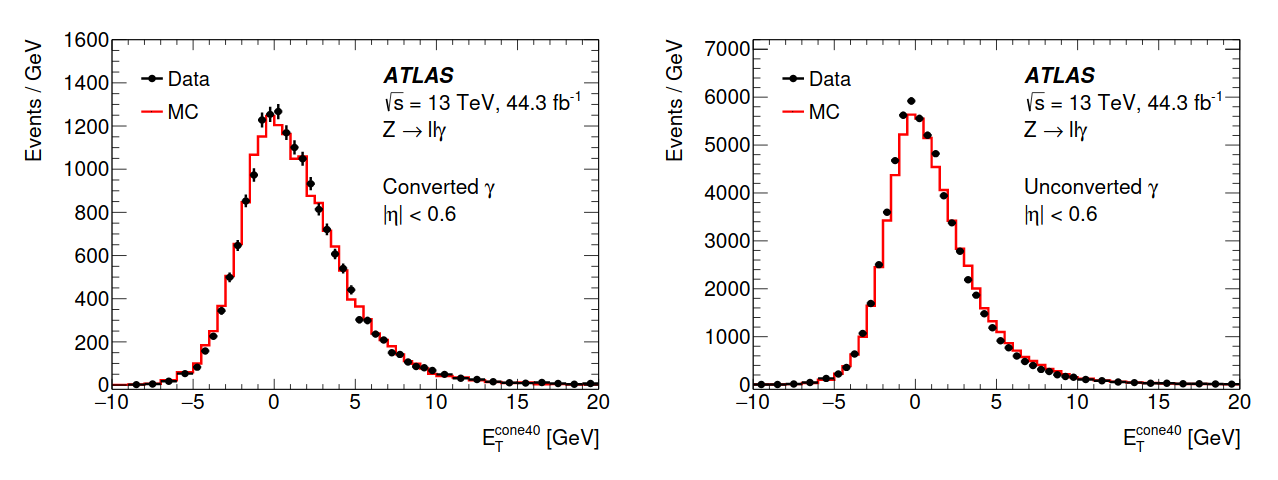
\includegraphics[width=0.85\textwidth]{Ch3/Img/photon_shifts_iso.png}
    \caption{Distribution of $E^{cone40}_T$ in data and simulation, in the central region of the detector ($|\eta|<$0.6), separately for converted (left) and unconverted (right) photons after the data-driven shifts are applied.}
    \label{fig:gamma:Iso:Shifts}
\end{figure}

Figure \ref{fig:gamma:Iso:Eff} shows the efficiency of the isolation working points defined in Table \ref{tab:gamma:Iso:WPs}, using $Z\rightarrow ll\gamma \ (l=e,\mu)$. The radiative Z decays signature is used to estimate the photon efficiencies since it provides a clean environment of prompt photons, especially in the low-\eT range. 
\begin{figure}[H]
    \centering
    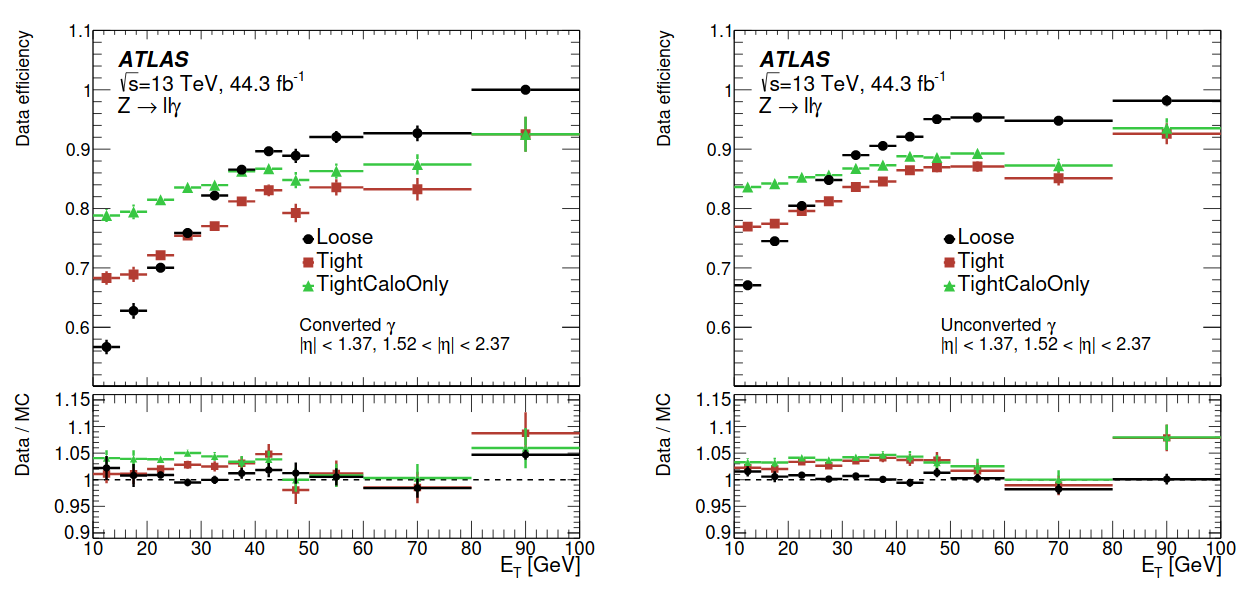
\includegraphics[width=0.85\textwidth]{Ch3/Img/Photon_Iso_Eff.png}
    \caption{Efficiency of the isolation working points for converted(left) and unconverted (right) photons as a function of photon \eT. The lower panel shows the ratio of the efficiencies measured in data and in simulation (scale factors).}
    \label{fig:gamma:Iso:Eff}
\end{figure}
\section{Photons Identification}
\label{gamma:ID}
\textcolor{red}{
The identification algorithm will be discussed here, and how the shower shape mis-modelling is affecting the ID efficiency. \\
}
In contrary to electron identification, photon identification still relies on rectangular selection criteria, \emph{cut-based algorithm}, using a set of global variables which characterize the lateral and longitudinal electromagnetic shower development in the calorimeter and encode separation between prompt-photons and fake photons originating from the decay of QCD jets. Such variables, listed in Table \ref{tab:chap2:Objects:Egamma:SS} and depicted in Figure \ref{fig:gamma:ID:SS} with their respective definitions, are called shower shapes. Shower shapes from the first EM layer play a significantly important role in rejecting the collimated photons from $\pi^0\rightarrow\gamma\gamma$ decay. \\ 
\begin{figure}[ht]
    \centering
    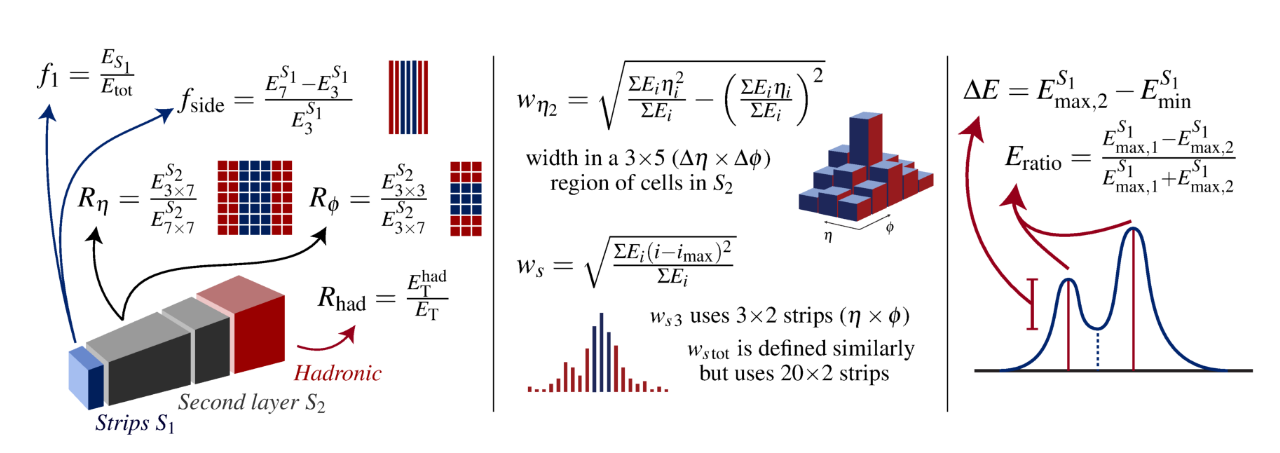
\includegraphics[width=0.85\textwidth]{Ch3/Img/ShowerShapes.png}
    \caption{Schematic representation of the photon identification discriminating variable \cite{ShowerShapes_fig}. \\}
    \label{fig:gamma:ID:SS}
\end{figure}
The cut-based algorithm provides three WPs: Tight, Medium and Loose, with less restrictive selections respectively. The Medium and Loose WPs mainly used for Trigger purposes. Since the trigger system is transparent between converted and unconverted photons, they are similar for both converted and unconverted. Table \ref{tab:gamma:ID:Var} lists the variables set used in each WP. The optimization of the WPs is done using TMVA \cite{TMVA} in bins of $|\eta|$ since the shower shapes vary due to calorimeter granularity. Because the shower shapes are different between the converted and unconverted photons due to the opening angle of the $e^+e^-$ conversion pair and the material interaction, the optimization of Tight WP is preformed separately for converted and unconverted photons. The Tight WP comes with two versions: \eT-independent selection and the \eT-dependent tuned in separate bins of \eT. The tuning is done in two energy regimes with two different series of simulated dataset. For photon with 10$<$\eT$<$25 GeV, the $Z\rightarrow ll\gamma$ simulated sample is used to define the signal, while the corresponding background is derived from the $Z\rightarrow ll+jets$ simulated sample. Above \eT=25 GeV, the inclusive-photon production simulated sample is used as a signal, and the background is the dijet. The simulated samples are described in Section 3.1 and 3.2 of Ref. \cite{Egamma_Perf_2017}.    
\begin{table}[H]
    \centering
    \begin{tabular}{cc}
        Working Point & Variables set \\
        \hline \hline
        Loose & \Rhad, \Rhadone, \Reta \ and \wetatwo \\ 
        Medium & Loose + \Eratio \\ 
        Tight & Medium + \Rphi, \wthree, \wtot, \Fside, \DeltaE \ and \fI \\ \hline \hline
    \end{tabular}
    \caption{Discriminating variables used for Loose, Medium and Tight photon identification.}
    \label{tab:gamma:ID:Var}
\end{table}
Similarly to the calorimeter based variables for isolation, the shower shapes variables suffer from the mis-modelling of the EM shower. The mis-modelling is addressed using a data-driven correction similar to the one applied for isolation features. Corrections are applied as a simple shift to simulated values to align with the real data distributions. Shifts are derived using a $\chi^2$ minimization between the data and simulation in bins of $|\eta|$ and \eT as described in Ref \cite{Photon_Eff_2015}. Figure \ref{fig:gamma:ID:SS:Corr} shows examples of the shower shapes distributions before and after correction compared to the real distributions using radiative Z photons. Section \ref{gamma:ss} dedicated to the shower shape mis-modelling and its correction using an alternative method. \\
\begin{figure}[ht]
    \centering
    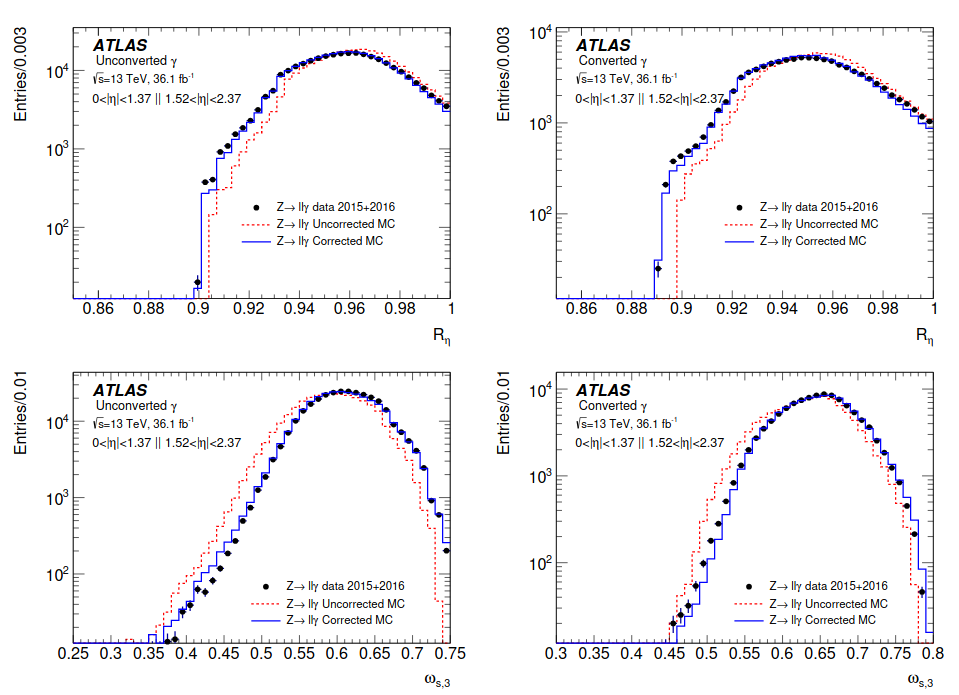
\includegraphics[width=0.75\textwidth]{Ch3/Img/SS_correction.png}
    \caption{Distributions of the \Reta \ and \wthree \ for converted and unconverted photon candidates with \eT in [10,50] GeV and $|\eta|<$2.37 selected from radiative Z events for data (black), uncorrected simulation (dashed red line) and the corrected simulation (solid blue line).}
    \label{fig:gamma:ID:SS:Corr}
\end{figure}
The photon identification efficiency is measured using three different methods over distinct energy regimes:
\begin{itemize}
\item The Matrix Method (MM) uses the inclusive-photon production sample collected using single-photon triggers and performed over a wide kinematic range from 25 GeV and up to 1.5 TeV. 
\item The Radiative Z method uses the clean signature of radiative Z at low-energy, allows a measurement of identification efficiency $\epsilon_{ID}$ from \eT=10 GeV up to 100 GeV. This method handles small background contamination from Z+jets where the jet is misidentified as photon using a maximum-likelihood fit \cite{Photon_Eff_Run1}. 
\item Electron Extrapolation (EE) is the third method, uses a transformed electron shower shapes sample form $Z\rightarrow e^+e^-$ and measures $\epsilon_{ID}$ in the region 25 $<$\eT$<$150 GeV.
\end{itemize}
These methods are fully described in Section 5 of Ref. \cite{Photon_Eff_2015}. The efficiencies from each method are then combined to provide a $\epsilon_{ID}$ measurement for the \eT-dependent selection as shown in Figures \ref{fig:gamma:ID:Eff:UnCov} and \ref{fig:gamma:ID:Eff:Cov}. 
\begin{figure}[ht]
    \centering
    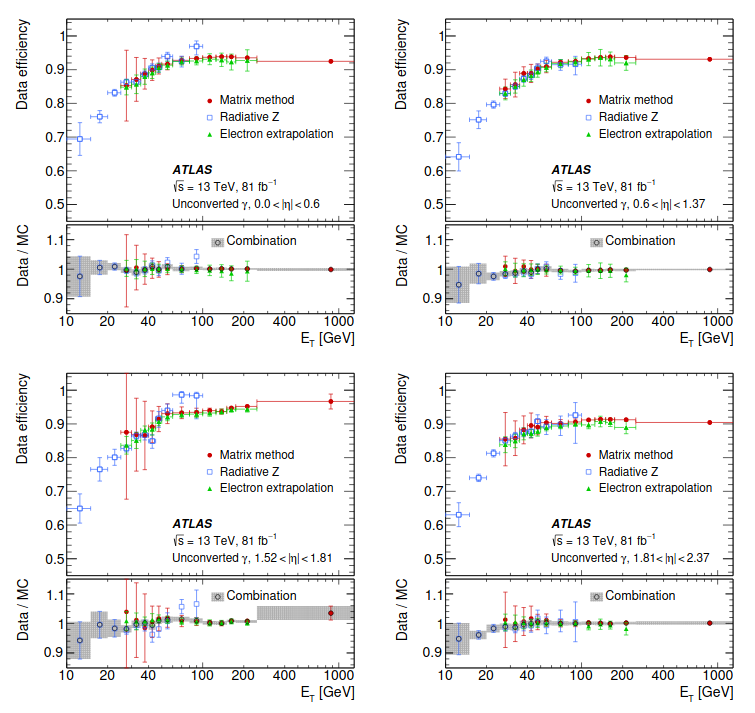
\includegraphics[width=0.6\textwidth]{Ch3/Img/Unconverted_Eff_2017.png}
    \caption{The photon identification efficiency with \eT-dependent selection, and the ratio of data to simulation efficiencies, for unconverted photons with a Loose isolation requirement applied as pre-selection, as a function of \eT in four different $|\eta|$ regions. The combined scale factor, obtained using a weighted average of scale factors from the individual measurements, is also presented; the band represents the total uncertainty.}
    \label{fig:gamma:ID:Eff:UnCov}
\end{figure}
\begin{figure}[ht]
    \centering
    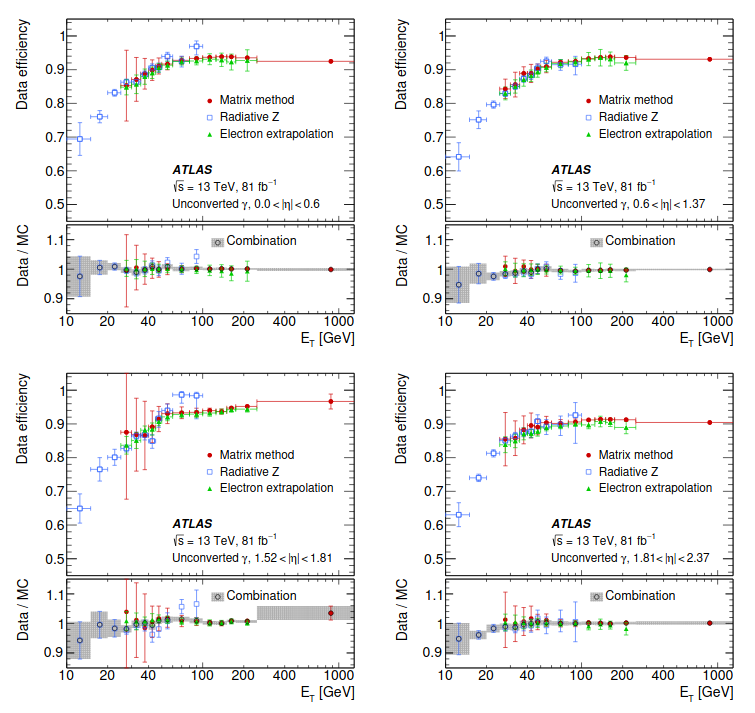
\includegraphics[width=0.6\textwidth]{Ch3/Img/Unconverted_Eff_2017.png}
    \caption{The photon identification efficiency with \eT-dependent selection, and the ratio of data to simulation efficiencies, for converted photons with a Loose isolation requirement applied as pre-selection, as a function of \eT in four different $|\eta|$ regions. The combined scale factor, obtained using a weighted average of scale factors from the individual measurements, is also presented; the band represents the total uncertainty.}
    \label{fig:gamma:ID:Eff:Cov}
\end{figure}
A comparison between the two versions of the Tight WP is shown in Figure \ref{fig:gamma:ID:Eff:Tight}.
\begin{figure}[ht]
    \centering
    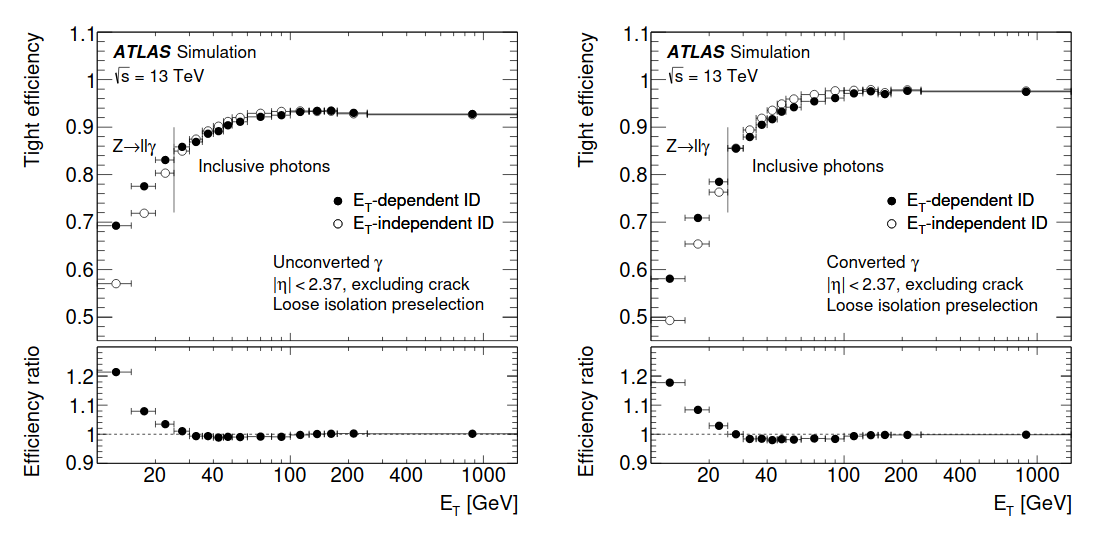
\includegraphics[width=0.75\textwidth]{Ch3/Img/Tight_ID.png}
    \caption{Efficiencies of the Tight photon identification for unconverted (left) and converted (right) signal photons, plotted as a function of photon \eT. The Loose isolation  is applied as a pre-selection. For both plots, the bottom panel shows the ratios between the \eT-dependent and the \eT-independent identification efficiencies.}
    \label{fig:gamma:ID:Eff:Tight}
\end{figure}
\textbf{The pile-up effect can fit with the CNN part}
\section{Shower shape mis-modelling}
\label{gamma:ss}
\textcolor{red}{The QT work will fit here. \\} 
The source of the disagreement in shower shapes between the data and simulation described above is remaining not clear. Many sources can contribute to this mis-modelling, mainly from the detector geometry, material distribution and EM shower modelling. It is hard to handle those sources and fix the mis-modelling. Indeed a cell-based reweighting method has been developed for electrons to apply a global correction in order to reduce systematic uncertainties related the mis-modelling. The approach shows a promising electron result, which makes its application also interesting to photons. This work is done in the context of my ATLAS qualification task for ATLAS authorship.
\subsection{Cell-based reweighting correction}
\label{gamma:ss:reweighting}
The aim is to redistribute the energy between the cluster cells in simulation to becomes consistent with the real data. The cell-based reweighting is derived for the second layer of the EM calorimeter. A cluster of 7x11 (7 cells in $\eta$ and 11 cells in $\phi$) centred around the cell with the highest energy (hottest) is considered. The correction is derived as a matrix (7x11) in bins of $\eta$ in two steps:
\begin{enumerate}
    \item Compute single cell corrections as : 
    \begin{equation}
        M_{i}^{Correction} = \frac{E_{i}^{data}}{\sum E_{i}^{data}} -  \frac{E_{i}^{simulated}}{\sum E_{i}^{simulated}}.
    \end{equation}
    Where $ E_{i = 1.. 77}$ denotes the cell energy in the 7x11 cluster of layer 2. 
    \item Compute the reweighted energy for each cluster cell as : 
    \begin{equation}
        E_{i}^{Reweighted} = E_{i}^{non-reweighted}(1+M_{i}^{Correction}).
    \end{equation}
\end{enumerate}
The main idea behind the reweighting is to factorize out the material effects and not the physics behaviours, especially the Bremsstrahlung tails in the energy profile for electrons and positrons. For electron only, the bremsstrahlung tails are extracted from the $e^+$ and $e^-$ energy profiles as: 
\begin{equation}
    E_{i} = (E_{i}^{electron} <  E_{i}^{positron}) \ ? \ E_{i}^{electron} \ : \  E_{i}^{positron},
\end{equation}
so it is derived independent from bremsstrahlung and similar for both electrons and positrons.
\subsection{Electron results}
Figure \ref{fig:gamma:ss:reweighting:electron} shows a reduction in data-simulation discrepancy after the reweighting and leads on a similar distribution for shower shape computed from layer 2 ($R_{\eta}$ and $R_{\phi}$) between data and simulation.
\begin{figure}[ht]
    \centering
    \subfloat[][]{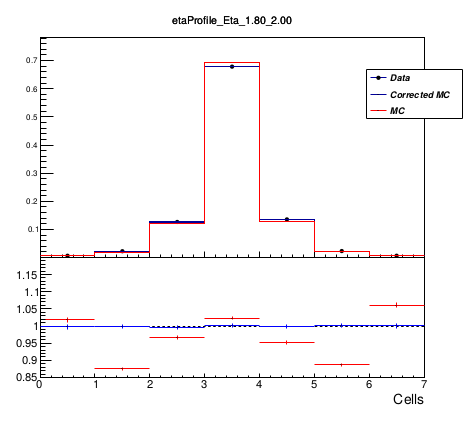
\includegraphics[width=.35\textwidth]{Ch3/Img/etaProfile_Reweighted_Zee.png}}
    \subfloat[][]{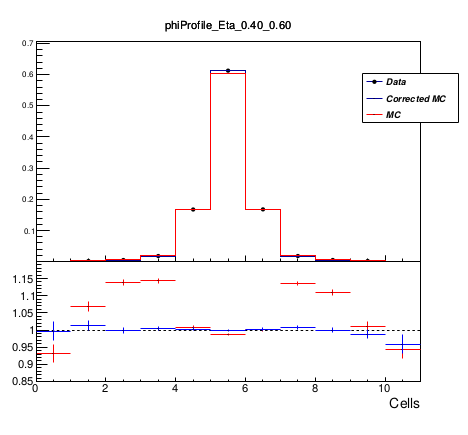
\includegraphics[width=.35\textwidth]{Ch3/Img/phiProfile_Reweighted_Zee.png}} \\
	\subfloat[][]{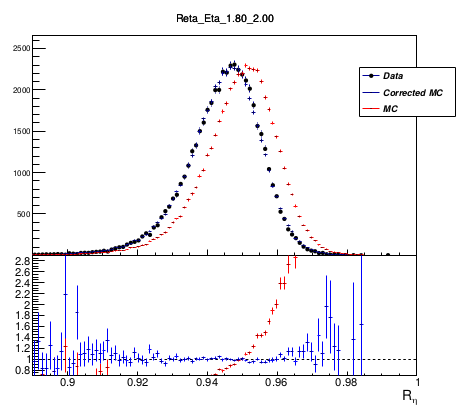
\includegraphics[width=.35\textwidth]{Ch3/Img/Reta_Reweighted_Zee.png}}
	\subfloat[][]{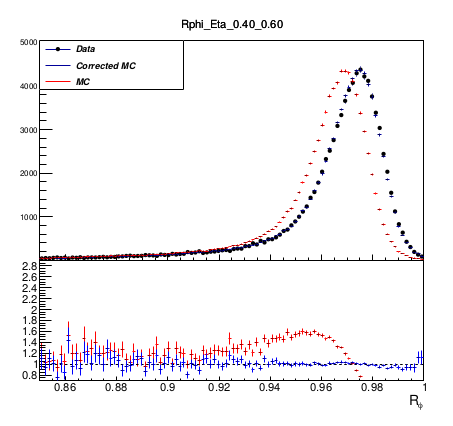
\includegraphics[width=.35\textwidth]{Ch3/Img/Rphi_Reweighted_Zee.png}}
    \caption{(a) Energy profile in $\eta$ direction, (b) Energy profile in $\phi$ direction, (c) $R_{\eta}$ variable and (d) $R_{\phi}$ variable before (red) and after reweighting for electrons from $Z\rightarrow e^+e^-$ for 1.80$<|\eta|<$2.00 first column and 0.40$<|\eta|<$0.60 in the second column (the bottom plot is the data/simulation ratio).}
    \label{fig:gamma:ss:reweighting:electron}
\end{figure}
The cell-based reweighting seems to be promising to reduce data-simulation mis-modelling on electrons shower shapes. Applying the same strategy to photons is interesting. 
\subsection{Cell-based reweighting for photons}
\label{gamma:ss:reweighting:photon}
\subsubsection{Event selection}
\label{gamma:ss:reweighting:photon:RadZSel}
For this study, Inclusive photons from the $Z\rightarrow ll\gamma$ are considered. The \verb|SHERPA| generator is used for simulated samples while the data correspond to the 2017 proton-proton collisions. The selection criteria applied are the following:
\begin{enumerate}
    \item Photon selection :  
    \begin{itemize}
    \item Transverse momentum $p_T > $  10 GeV.
    \item Pseudorapidity $|\eta|$ within the calorimeter acceptance : $|\eta| < $ 2.37, excluding the transition region between the barrel and end-cap (crack region) : 1.37 $ < |\eta| < $ 1.52
    \item Isolation : Tight WP.
    \item Identification : None. 
\end{itemize}
    \item Electron selection :
    \begin{itemize}
        \item Transverse momentum $p_T > $ 10 GeV.
        \item Pseudorapidity $|\eta| < $ 1.37 or $1.52 < |\eta| < $ 2.47.
        \item Longitudinal impact parameter $z_0 < $ 10 mm, transverse impact parameter significance $|d_0|/\sigma_{d_0} < $ 10.
        \item Isolation : Loose WP.
        \item Identification : Medium.
    \end{itemize}
    \item Combined Muon selection : 
    \begin{itemize}
        \item Transverse momentum $p_T > $ 10 GeV.
        \item Pseudorapidity $|\eta| < $ 2.5.
        \item Longitudinal impact parameter $z_0 < $ 10 mm, transverse impact parameter significance $|d_0|/\sigma_{d_0} < $ 10.
        \item Isolation : Loose WP.
        \item Identification : Medium WP.
    \end{itemize}
    \item $Z \rightarrow ll\gamma$ event selection :
    \begin{itemize}
        \item $\Delta R_{min}(e,\gamma) > $ 0.4 and $\Delta R_{min}(\mu,\gamma) > $ 0.2: the selection is tighter for electron channel to reduce photon from electron bremsstrahlung.
        \item 80 $ < m_{ll\gamma} < $ 100 GeV to select Z peak,  and 40 $ < m_{ll} < $ 83 GeV for final state radiation (FSR) event selection. 
    \end{itemize}
\end{enumerate}
No identification criteria is applied to photons to avoid any bias from the identification.
\subsubsection{Electrons reweighting applied to photons}
The first strategy has been to apply the electron reweighting to photons. The developed reweighting matrix for electrons is directly applied to the selected photons from radiative Z events. Figure \ref{fig:gamma:ss:reweighting:photon:electron} shows the energy profiles and layer 2 shower shapes variables before and after the reweighting. The reweighting goes in the correct direction but not enough to correct photons shower shape mis-modelling; this motivates to implement specific reweighting for photons. Additional control plots for other $\eta$ regions and converted photons are provided in Appendix ().
\begin{figure}[ht]
    \centering
	\subfloat[][]{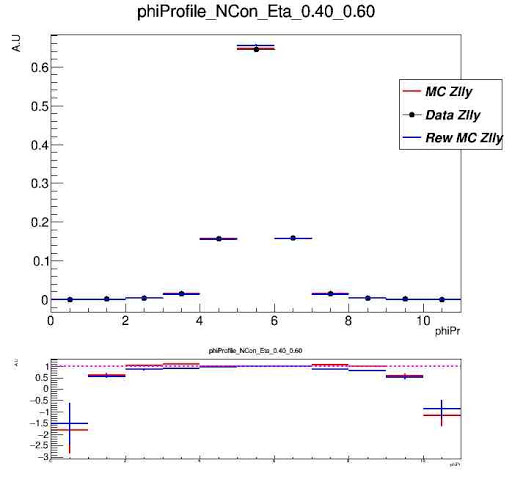
\includegraphics[width=.35\textwidth]{Ch3/Img/phiProfile_NCon_Eta_0.40_0.60.jpg}}
	%\subfloat[][]{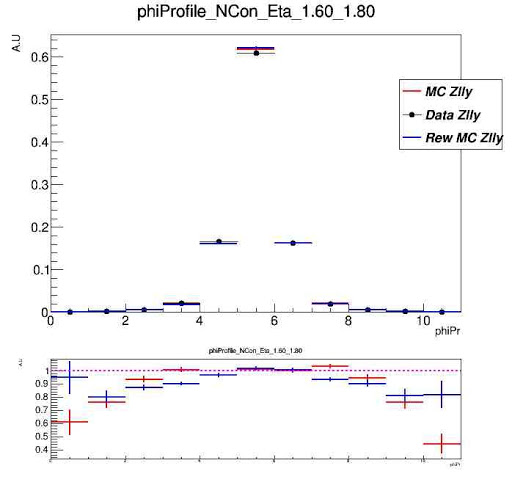
\includegraphics[width=.25\textwidth]{Ch3/Img/phiProfile_NCon_Eta_1.60_1.80.jpg}} 
	%\subfloat[][]{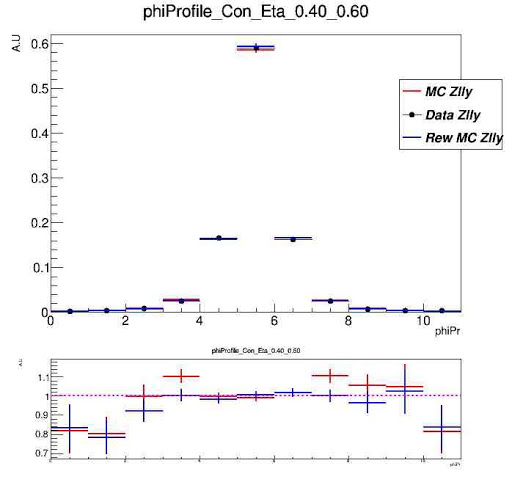
\includegraphics[width=.25\textwidth]{Ch3/Img/phiProfile_Con_Eta_0.40_0.60.jpg}}
	%\subfloat[][]{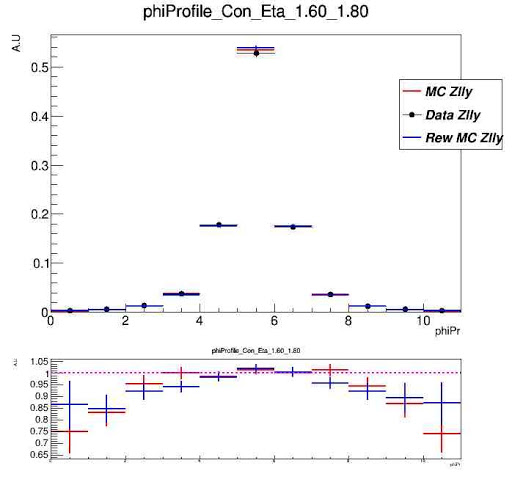
\includegraphics[width=.25\textwidth]{Ch3/Img/phiProfile_Con_Eta_1.60_1.80.jpg}} \\
	\subfloat[][]{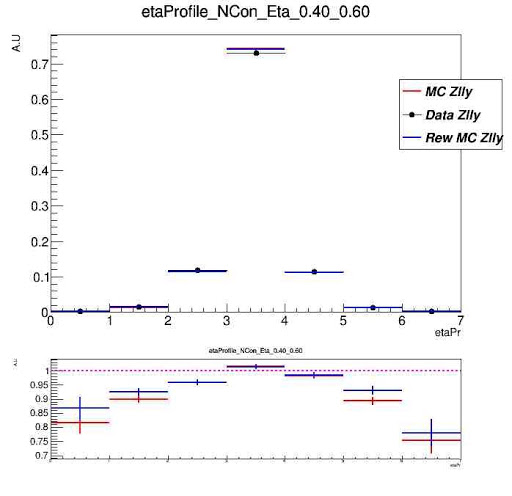
\includegraphics[width=.35\textwidth]{Ch3/Img/etaProfile_NCon_Eta_0.40_0.60.jpg}} \\
	%\subfloat[][]{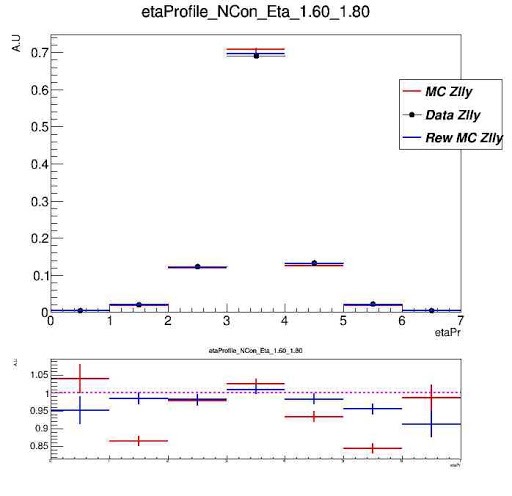
\includegraphics[width=.25\textwidth]{Ch3/Img/etaProfile_NCon_Eta_1.60_1.80.jpg}} 
	%\subfloat[][]{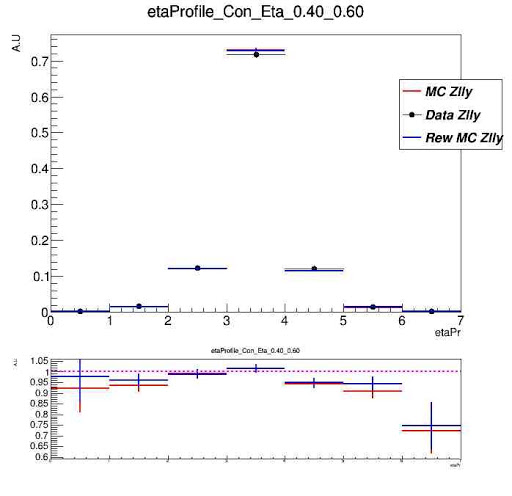
\includegraphics[width=.25\textwidth]{Ch3/Img/etaProfile_Con_Eta_0.40_0.60.jpg}}
	%\subfloat[][]{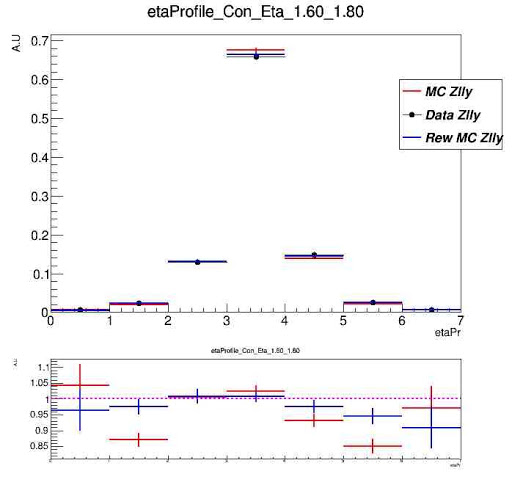
\includegraphics[width=.25\textwidth]{Ch3/Img/etaProfile_Con_Eta_1.60_1.80.jpg}} \\
	\subfloat[][]{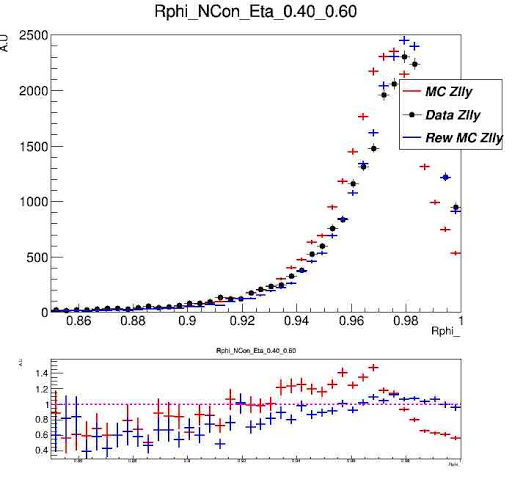
\includegraphics[width=.35\textwidth]{Ch3/Img/Rphi_NCon_Eta_0.40_0.6.jpg}}
	%\subfloat[][]{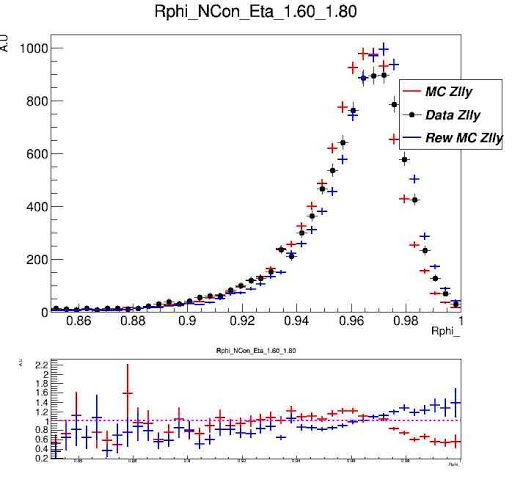
\includegraphics[width=.25\textwidth]{Ch3/Img/Rphi_NCon_Eta_1.60_1.80.jpg}}
	%\subfloat[][]{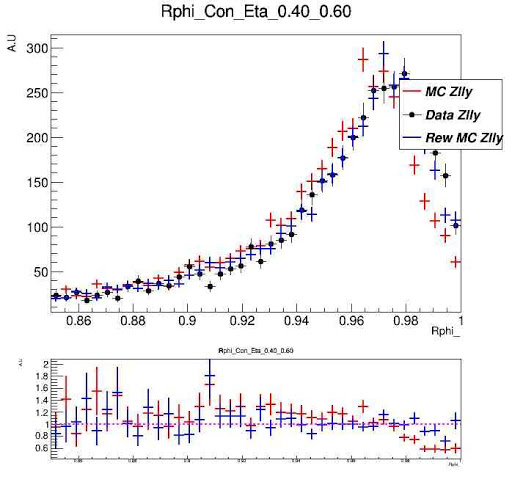
\includegraphics[width=.25\textwidth]{Ch3/Img/Rphi_Con_Eta_0.40_0.6.jpg}}
	%\subfloat[][]{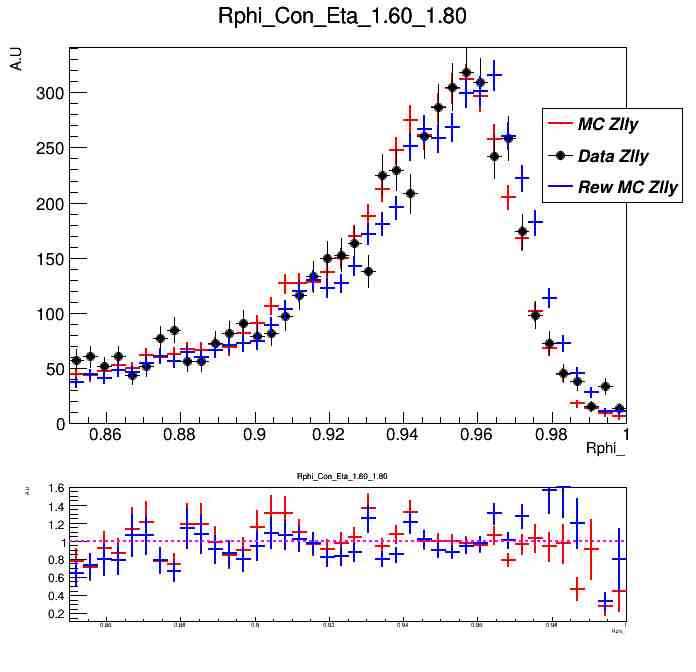
\includegraphics[width=.25\textwidth]{Ch3/Img/Rphi_Con_Eta_1.60_1.80.jpg}} \\
	\subfloat[][]{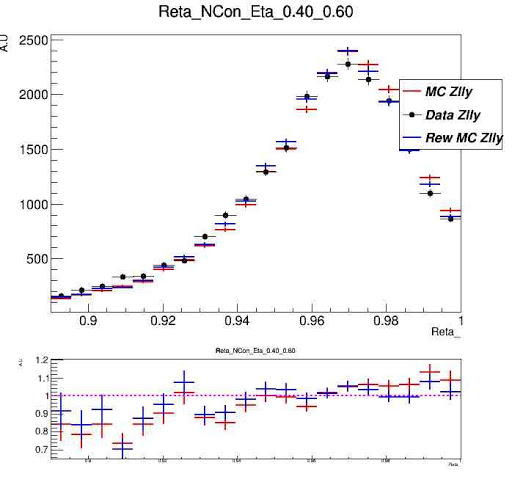
\includegraphics[width=.35\textwidth]{Ch3/Img/Reta_NCon_Eta_0.40_0.6.jpg}}
	%\subfloat[][]{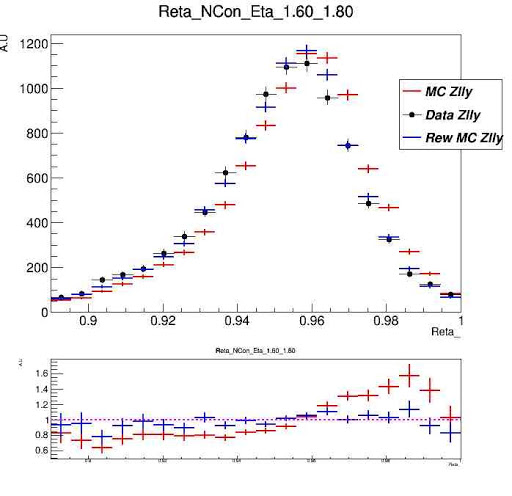
\includegraphics[width=.25\textwidth]{Ch3/Img/Reta_NCon_Eta_1.60_1.80.jpg}}
	%\subfloat[][]{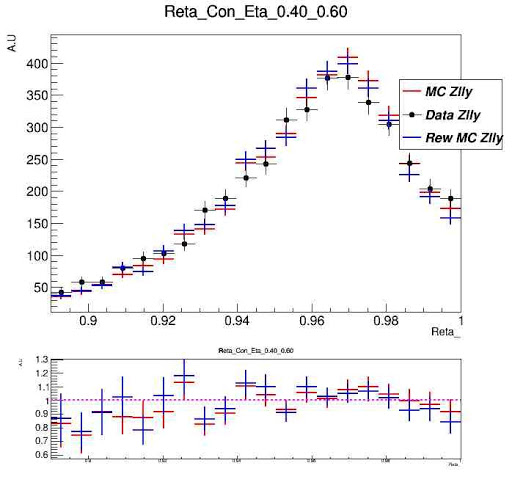
\includegraphics[width=.25\textwidth]{Ch3/Img/Reta_Con_Eta_0.40_0.6.jpg}}
	%\subfloat[][]{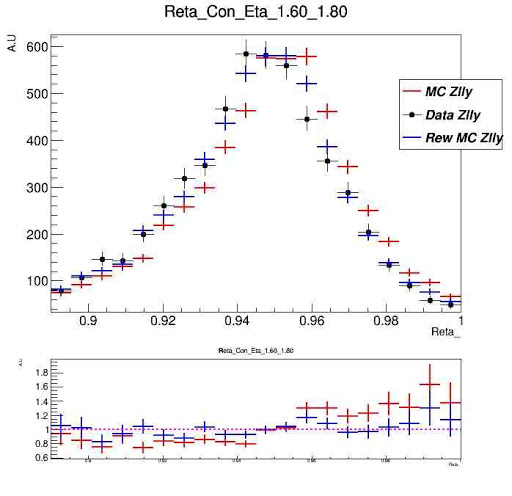
\includegraphics[width=.25\textwidth]{Ch3/Img/Reta_Con_Eta_1.60_1.80.jpg}}
    \caption{The energy profile in $\phi$ and $\eta$ directions (a,b) and the corresponding \Rphi and \Reta variables, for unconverted photons with 0.40$<|\eta|<$0.60. The black points correspond to Data 2017, red points to non-reweighted simulation and blue points to the reweighted simulation from $Z\rightarrow ll\gamma$.}
    \label{fig:gamma:ss:reweighting:photon:electron}
\end{figure}
\subsubsection{Photon reweighting}
The second strategy is to drive specific reweighting for photon. Similarly to electrons, the reweighting is recomputed for photons using radiative Z events inclusively in conversion to allow for more statistics. Figure \ref{fig:gamma:ss:reweighting:photon:photon} shows the profiles and shower shapes after applying the derived reweighting on photons. A good agreement is observed in energy profiles for both direction $\eta$ and $\phi$. However for shower shapes variables, no significant improvement is observed and the reweighting seems to be not working for photons. From the energy profiles in Figures \ref{fig:gamma:ss:reweighting:photon:electron} and \ref{fig:gamma:ss:reweighting:photon:photon} photons reweighting from radiative Z are larger than the one for electrons. Additional control plots for other $\eta$ regions and converted photons are provided in Appendix (). To validate the reweighting procedure a closure test is performed on pseudo data.
\begin{figure}[ht]
    \centering
	\subfloat[][]{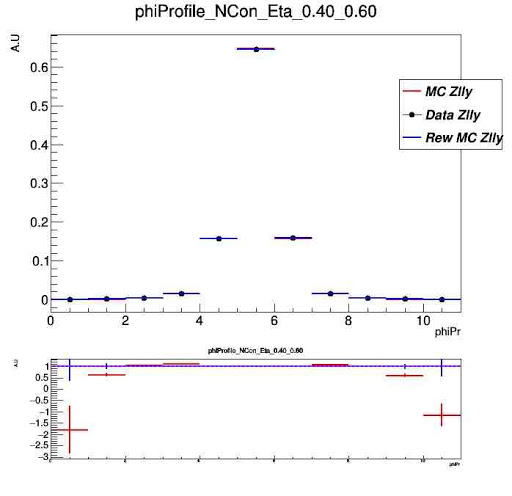
\includegraphics[width=.35\textwidth]{Ch3/Img/PhotonRew/phiProfile_NCon_Eta_0.40_0.60.jpg}}
	%\subfloat[][]{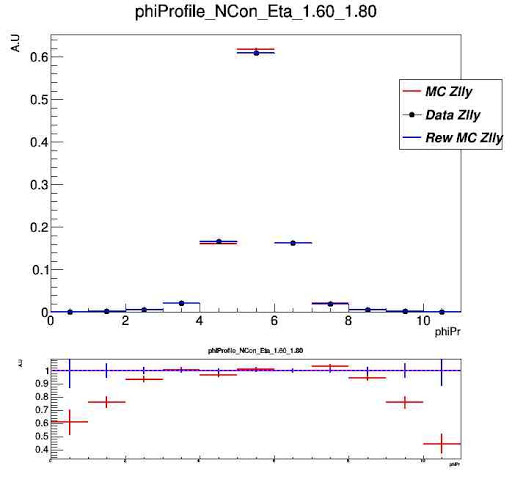
\includegraphics[width=.25\textwidth]{Ch3/Img/PhotonRew/phiProfile_NCon_Eta_1.60_1.80.jpg}} 
	\subfloat[][]{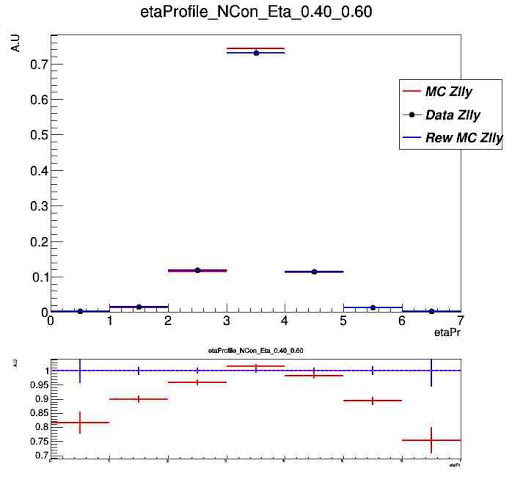
\includegraphics[width=.35\textwidth]{Ch3/Img/PhotonRew/etaProfile_NCon_Eta_0.40_0.60.jpg}} \\
	%\subfloat[][]{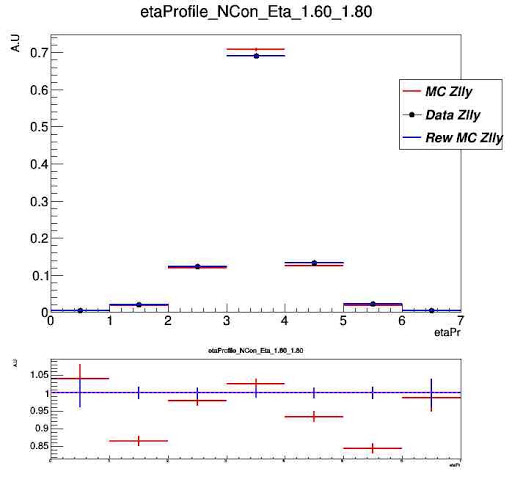
\includegraphics[width=.25\textwidth]{Ch3/Img/PhotonRew/etaProfile_NCon_Eta_1.60_1.80.jpg}} \\
	\subfloat[][]{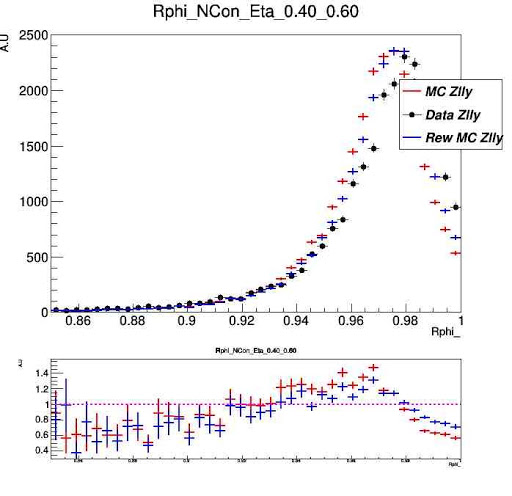
\includegraphics[width=.35\textwidth]{Ch3/Img/PhotonRew/Rphi_NCon_Eta_0.40_0.60.jpg}}
	%\subfloat[][]{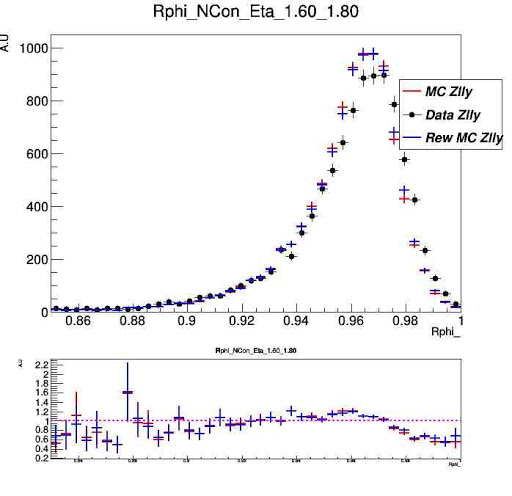
\includegraphics[width=.25\textwidth]{Ch3/Img/PhotonRew/Rphi_NCon_Eta_1.60_1.80.jpg}}
	\subfloat[][]{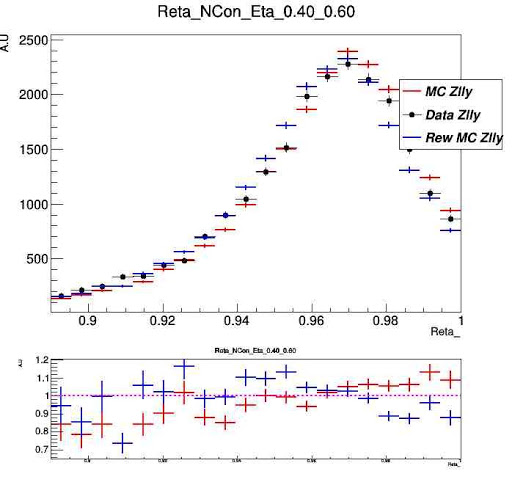
\includegraphics[width=.35\textwidth]{Ch3/Img/PhotonRew/Reta_NCon_Eta_0.40_0.60.jpg}}
	%\subfloat[][]{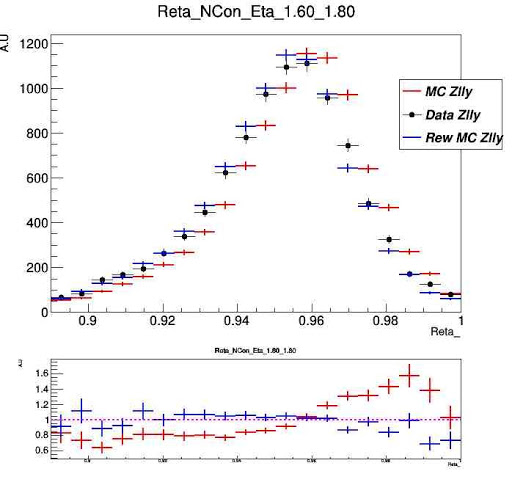
\includegraphics[width=.25\textwidth]{Ch3/Img/PhotonRew/Reta_NCon_Eta_1.60_1.80.jpg}}
    \caption{The energy profile in $\phi$ and $\eta$ directions (a,b) and the corresponding \Rphi and \Reta variables, for unconverted photons with 0.40$<|\eta|<$0.60. The black points correspond to Data 2017, red points to non-reweighted simulation and blue points to the reweighted simulation from $Z\rightarrow ll\gamma$.}
    \label{fig:gamma:ss:reweighting:photon:photon}
\end{figure}
\subsubsection{Closure test}
To evaluate the reduction in discrepancy between data and simulation, a closure test is performed using pseudo data (PS) from simulation, for that :
\begin{enumerate}
    \item Pseudo data is produced by adding 50 MeV (arbitrary value) to each simulated cell.
    \item Re-compute the reweighting function with the same procedure as above using unconverted photons (for simplicity).
    \item Correct simulated cell to match the pseudo data.
\end{enumerate}
Results of the closure test are shown in Figure \ref{fig:gamma:ss:reweighting:photon:closure}. 
\begin{figure}[ht]
    \centering
	\subfloat[][]{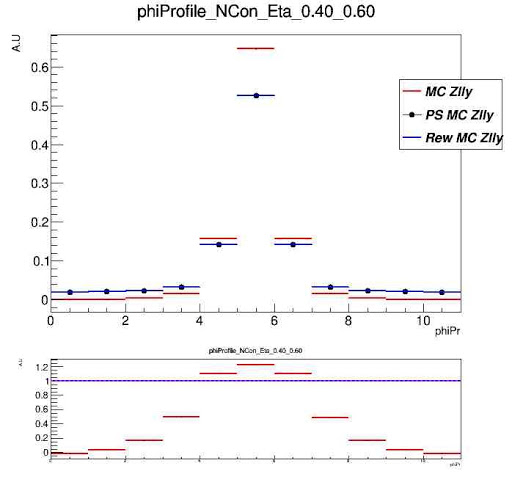
\includegraphics[width=.35\textwidth]{Ch3/Img/PhotonRew/PS_phiProfile_NCon_Eta_0.40_0.60.jpg}}
	%\subfloat[][]{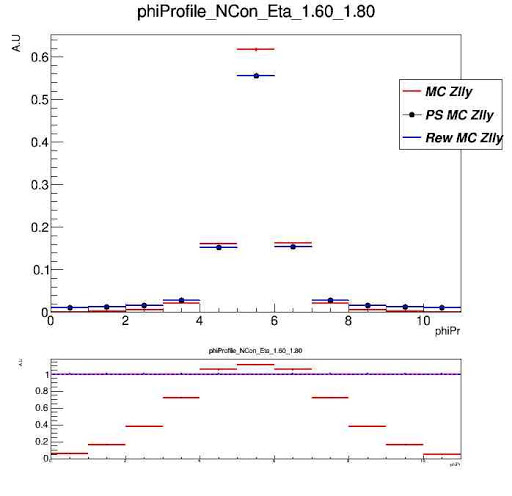
\includegraphics[width=.25\textwidth]{Ch3/Img/PhotonRew/PS_phiProfile_NCon_Eta_1.60_1.80.jpg}}
	\subfloat[][]{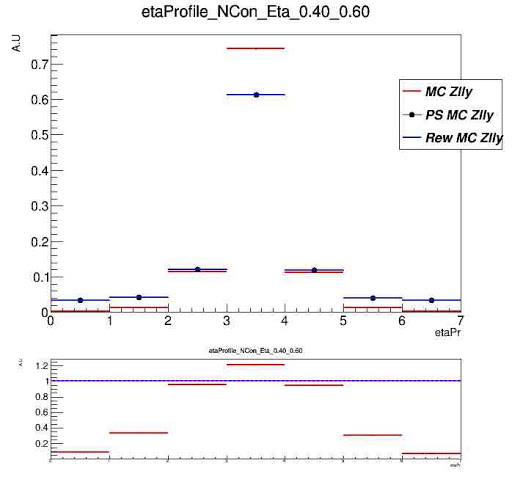
\includegraphics[width=.35\textwidth]{Ch3/Img/PhotonRew/PS_etaProfile_NCon_Eta_0.40_0.60.jpg}} \\
	%\subfloat[][]{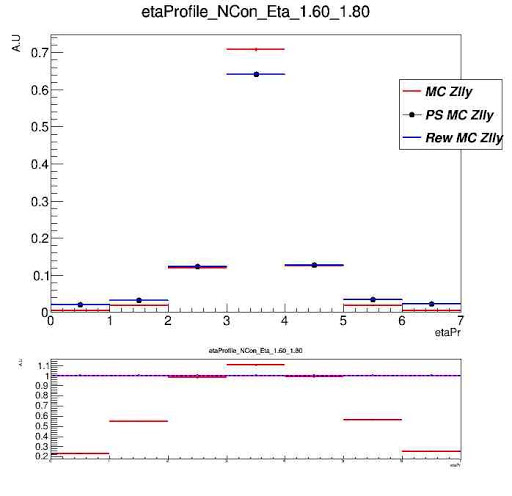
\includegraphics[width=.25\textwidth]{Ch3/Img/PhotonRew/PS_etaProfile_NCon_Eta_1.60_1.80.jpg}} \\
	\subfloat[][]{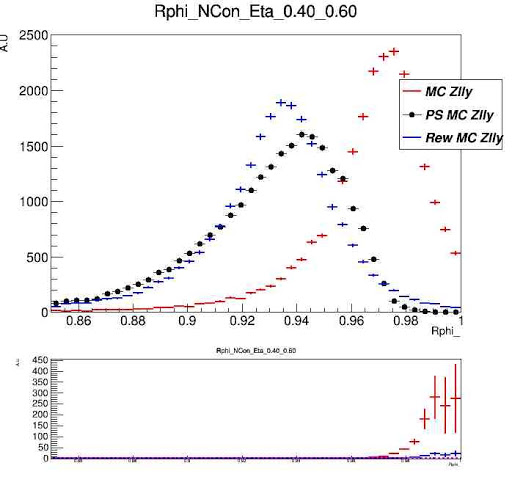
\includegraphics[width=.35\textwidth]{Ch3/Img/PhotonRew/PS_Rphi_NCon_Eta_0.40_0.60.jpg}}
	%\subfloat[][]{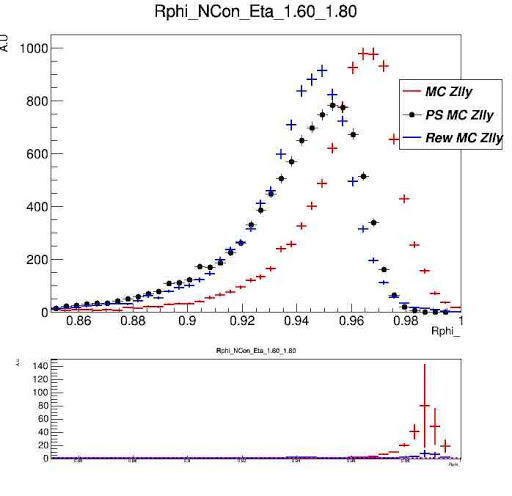
\includegraphics[width=.25\textwidth]{Ch3/Img/PhotonRew/PS_Rphi_NCon_Eta_1.60_1.80.jpg}}
	\subfloat[][]{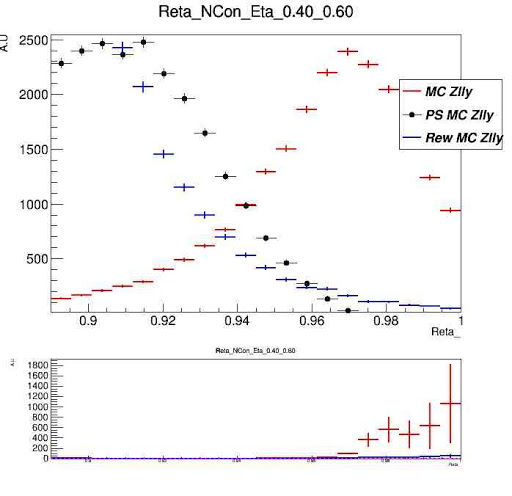
\includegraphics[width=.35\textwidth]{Ch3/Img/PhotonRew/PS_Reta_NCon_Eta_0.40_0.60.jpg}}
	%\subfloat[][]{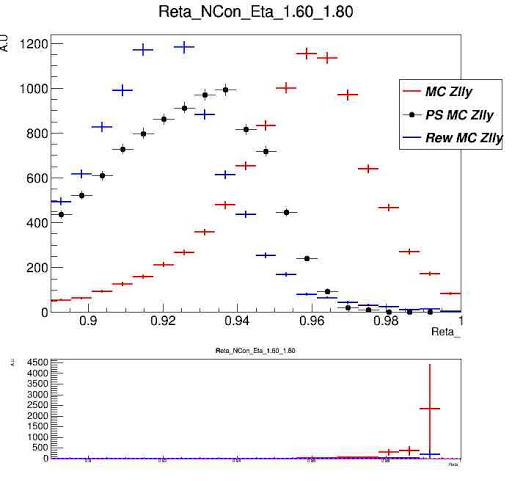
\includegraphics[width=.25\textwidth]{Ch3/Img/PhotonRew/PS_Reta_NCon_Eta_1.60_1.80.jpg}}
    \caption{The energy profile in $\phi$ and $\eta$ directions (a,b) and the corresponding \Rphi and \Reta variables, for unconverted photons with 0.40$<|\eta|<$0.60. The black points correspond to the pseudo data, red points to non-reweighted simulation and blue points to the reweighted simulation from $Z\rightarrow ll\gamma$.}
    \label{fig:gamma:ss:reweighting:photon:closure}
\end{figure}
Perfect agreement in energy profiles for both directions ($\eta$ and $\phi$) is observed, the closure test reproduces the pseudo data, while for shower shapes the agreement is improved in the correct direction but not enough to correct the fake mis-modelling. The closure test shows that the reweighting procedure was not able to catch the discrepancy between data and simulation, and seems to be working only on average and not event-by-event. Figure \ref{fig:gamma:ss:reweighting:photon:closure:avg} shows the averages of $R_{\eta}$ and $R_{\phi}$ in real data, simulation and after reweighting in bin of photon $|\eta|$. After reweighting, the average of shower shapes in simulation perfectly matches the data distribution, which demonstrates that the reweighting is working on average and not event-by-event.

\begin{figure}[H]
    \centering
    \subfloat[][]{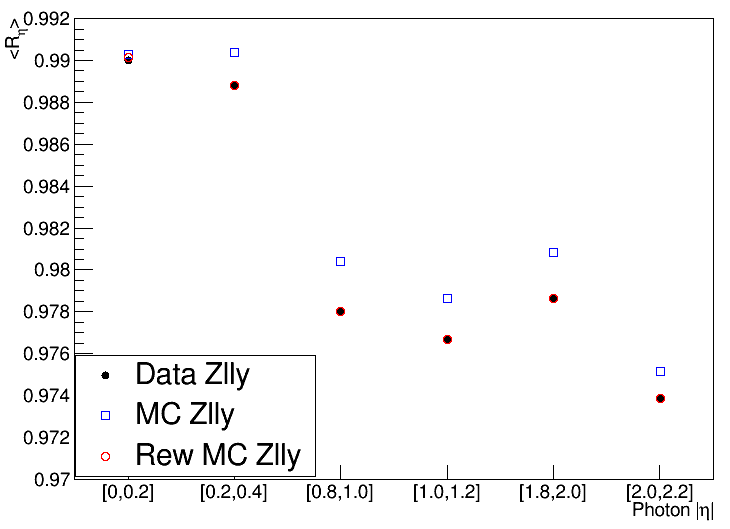
\includegraphics[width=.35\textwidth]{Ch3/Img/PhotonRew/Reta_avg.png}}
    \subfloat[][]{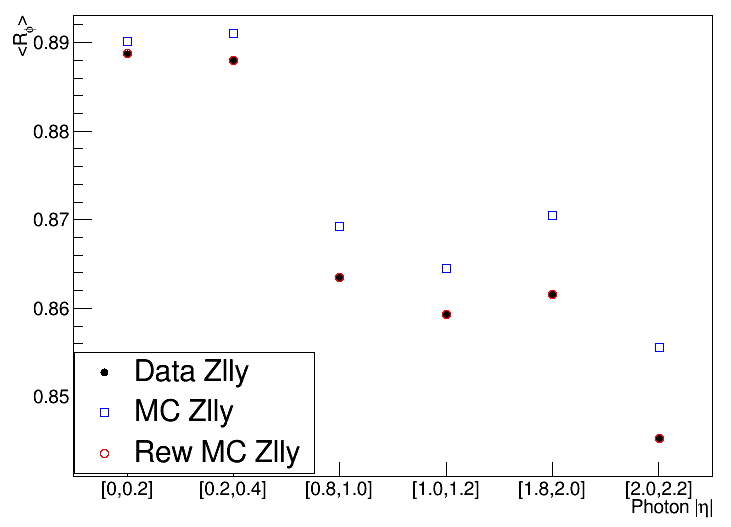
\includegraphics[width=.35\textwidth]{Ch3/Img/PhotonRew/Rphi_avg.png}}
    \caption{Average $R_{\eta}$ (a) and $R_{\phi}$ (b) in real data (black), simulation (blue) and after reweighting (red) using photon reweighting.}
    \label{fig:gamma:ss:reweighting:photon:closure:avg}
\end{figure}

\label{tab:avg}

%One of the possible reasons why reweighting works for electrons and not for photons is the fact that the reweighting function for electrons benefits from high statistics leads to modulate the energy in each cell with a Gaussian distribution (Central limits theorem) instead of photons which suffer from low statistics and high background contamination. Having more statistics and sophisticated techniques to extract background will helps to generate a reweighting function for photons.
\subsubsection{3-dimensional reweighting}
Since the reweighting is only working on average and not event-by-event, a new reweighting technique is presented here. The idea is to add cell energy as a dimension to the previous reweighting procedure. The reweighting factor for each cell will be a function of cell energy. Instead of 2D reweighting the reweighting will be in 3 dimensions, defined as:
\begin{equation}
    E_{k,n}^{Rew} = E_{k,n} \times \alpha \ ; with \ \alpha = f(k,n,E_{k,n}) = E_{k,n}^{Data}/E_{k,n}
\end{equation}
Where k = 1..77 denotes the cell number, n the corresponding photon $|\eta|$ bin and $E_{k,n}$ is the energy of cell k in $\eta$ bin n. \\
The new method requires a perfect matching between photons from data and MC to compute the $\alpha$ factors, which is technically complicated. The procedure is tested with PS data from MC. The PS data is derived from MC by scaling the energy of cell k by 0.26 (the factor 0.26 is arbitrary). For simplicity, the reweighting is evaluated using unconverted photons only.
The result of the new reweighting procedure is presented in Figure \ref{fig:gamma:ss:reweighting:photon:3dreweighting}. A good agreement is observed after the 3D reweighting for both energy profiles and their corresponding shower shapes variables for layer 2. The improvement in data-MC agreement observed makes the new method promising to be applied to real data.
%This work is kept for the newcomers to the ATLAS collaboration.
\begin{figure}[ht]
    \centering
	\subfloat[][]{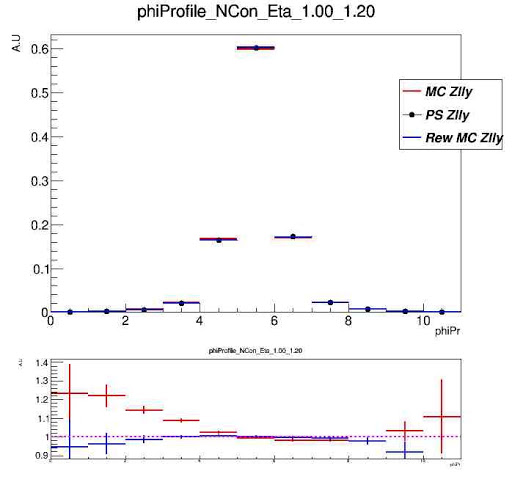
\includegraphics[width=.25\textwidth]{Ch3/Img/PhotonRew/NPS_phiProfile_NCon_Eta_1.0_1.20.jpg}}
	%\subfloat[][]{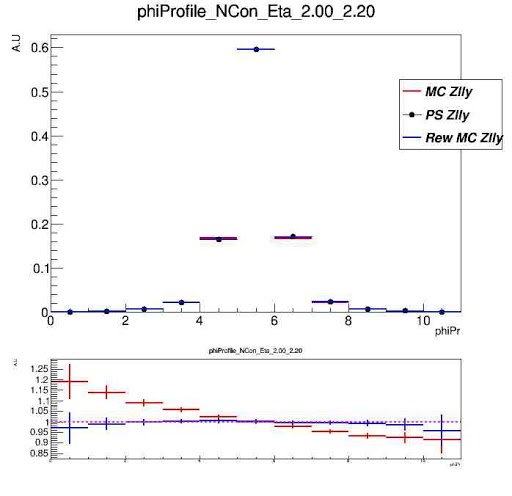
\includegraphics[width=.25\textwidth]{Ch3/Img/PhotonRew/NPS_phiProfile_NCon_Eta_2.20_2.40.jpg}}
	\subfloat[][]{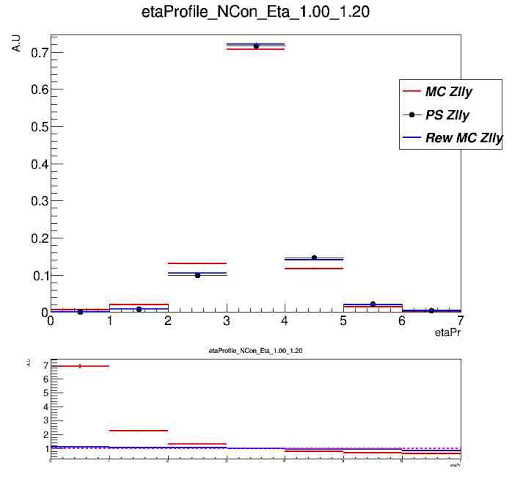
\includegraphics[width=.25\textwidth]{Ch3/Img/PhotonRew/NPS_etaProfile_NCon_Eta_1.0_1.20.jpg}} \\
	%\subfloat[][]{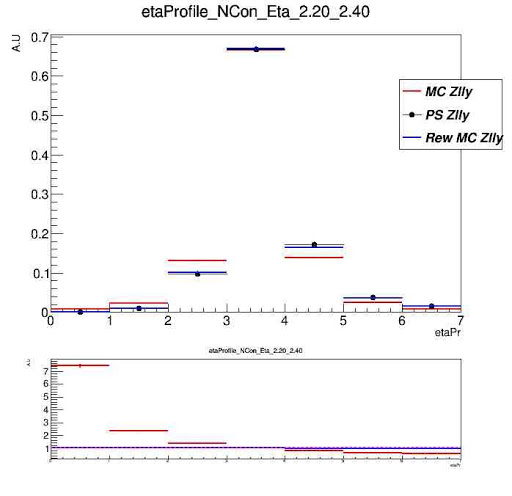
\includegraphics[width=.25\textwidth]{Ch3/Img/PhotonRew/NPS_etaProfile_NCon_Eta_2.20_2.40.jpg}} \\
	\subfloat[][]{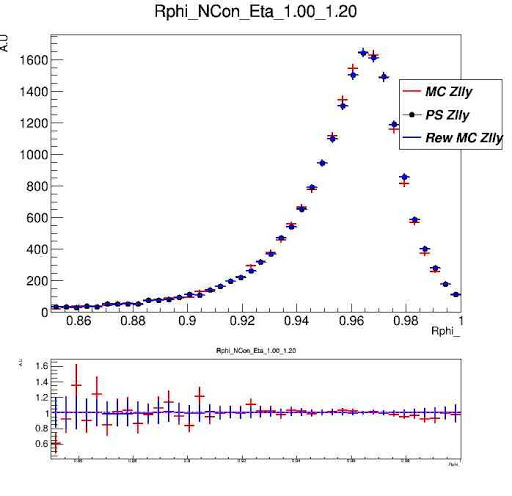
\includegraphics[width=.25\textwidth]{Ch3/Img/PhotonRew/NPS_Rphi_NCon_Eta_1.00_1.20.jpg}}
	%\subfloat[][]{\includegraphics[width=.25\textwidth]{Ch3/Img/PhotonRew/NPS_Rphi_NCon_Eta_2.00_2.20.jpg}}
	\subfloat[][]{\includegraphics[width=.25\textwidth]{Ch3/Img/PhotonRew/NPS_Reta_NCon_Eta_1.00_1.20.jpg}}
	%\subfloat[][]{\includegraphics[width=.25\textwidth]{Ch3/Img/PhotonRew/NPS_Reta_NCon_Eta_2.00_2.20.jpg}}
    \caption{The energy profile in $\phi$ and $\eta$ directions (a,b) and the corresponding \Rphi and \Reta variables, for unconverted photons with 1.00$<|\eta|<$1.20. The black points correspond to the pseudo data, red points to non-reweighted MC and blue points to the reweighted MC from $Z\rightarrow ll\gamma$.}
    \label{fig:gamma:ss:reweighting:photon:3dreweighting}
\end{figure}

\section{Convolutional Neural Network for Photon Identification}
\label{gamma:CNN}
\textcolor{red}{The CNN work will fit here to improve the photon identification efficiency and if scale factor are ready by the date of the thesis will be included to. \\}

Using shower shape variables for the identification algorithm limits the performance to learn the shower difference between prompt and fake photons. Correcting the mis-modelling seems to be a critical problem without any solution for the moment. For these reasons, a significant improvement is possible to achieve by developing a new identification algorithm based on the EM cells and using advance Machine Learning (ML) techniques. The EM cells of the photon cluster are commonly represented as an image, where each pixel contains the cell energy, leading to use of images of the deposited energy of the photon in the calorimeter to learn the shower properties. The most adapted ML technique for image processing is Convolutional Neural Networks (CNNs). In the following, we describe how we develop a CNN algorithm to improve the photon identification efficiency using EM calorimeter images. This section assumes knowledge of the NNs system from the reader. 
\subsubsection{Event selection}
Simulated samples of inclusive photon production are used to train the CNN. The inclusive photon sample includes $\gamma$+jet events from the hard subprocesses $qg \rightarrow q\gamma$ and $ q\bar{q}\rightarrow g\gamma$ enriched by prompt photon and used as a signal for the training. Fake photons (background) are toked from quark fragmentation in QCD di-jet events. Photon candidates are requested to pass the same photon selection defined for radiative Z in Section \ref{gamma:ss:reweighting:photon:RadZSel}. Additionally, photons used as a signal in the training (prompt) are required to be a stable particle, not originating from a hadron and match a truth photon. Photons failing one of these requirements are flagged as a background (fake). Photons from radiative Z decay are used as a control sample to evaluate the performance of the trained model (out-of-sample validation).
\subsubsection{Images pre-processing}
\label{gamma:CNN:PreProcessing}
To compromise between collecting more energy and being minimising the impact of the activity around the cluster, the 7x11 cluster around the hottest cell is considered similarly to the shower shapes computation. As the EM cell granularity changes with $\eta$ (Table \ref{tab:chap2:ATLAS:Calo:ECal:Gr}), it leads to different number of cells in each $\eta$ region and different sizes in the first sampling. The corresponding number of cells in 7x11 windows are summarized in Table \ref{tab:gamma:CNN:PreProcessing:NCells}.
\begin{table}[H]
    \centering
    \begin{tabular}{ccccc}
    \hline
        $|\eta|$ range & 0 to 1.4 & 1.4 to 1.8 & 1.8 to 2.0 & 2.0 to 2.5 \\
    \hline
        Sampling 1 & 112 & 112 & 84 & 56 \\
        Sampling 2 & 77 & 77 & 77 & 77 \\
        Sampling 3 & 44 & 44 & 44 & 44 \\
    \hline
    \end{tabular}
    \caption{Number of cells in 7x11 EM calorimeter windows.}
    \label{tab:gamma:CNN:PreProcessing:NCells}
\end{table}
The difference in shape and size of the EM calorimeter windows complicates the network training procedure. To avoid this issue, zeros are appended to the calorimeter cluster image to end up with the same image size in all $\eta$ region for each sampling (e.g sampling 1 with 84 cells is completed by zeros, to have 112 cells). Table \ref{tab:gamma:CNN:PreProcessing:ImgSize} shows the final image shape used for each sampling.
\begin{table}[H]
    \centering
    \begin{tabular}{cc}
    \hline
        Sampling & Shape \\
    \hline
        Sampling 1 & (56,2)\\
        Sampling 2 & (7,11)  \\
        Sampling 3 & (4,11) \\
    \hline
    \end{tabular}
    \caption{Image shape of 7x11 windows in each sampling in ($\eta$,$\phi$).}
    \label{tab:gamma:CNN:PreProcessing:ImgSize}
\end{table}
I decided to use the cell energy normalized to the total cluster energy as image pixel to build an energy independent algorithm which performs in the same way for all energy regime.
\subsubsection{CNN Architecture}
\label{gamma:CNN:Model}
A CNN classifier is built to separate between prompt and background photons using images of the 7x11 cluster windows of sampling 1, 2, and 3. Figure \ref{fig:gamma:CNN:Model:Idea} shows an illustration of the classifier.
\begin{figure}[H]
    \centering
    \includegraphics[width=.6\textwidth]{Ch3/Img/CNN_Idea.png}
    \caption{CNN classifier schema.}
    \label{fig:gamma:CNN:Model:Idea}
\end{figure}
The Global CNN classifier is constructed using the \textsc{Keras} library, with \textsc{Tensorflow} as a backend \cite{keras, tensorflow}. Information from EM layers images is extracted using three babies CNN. Each one is connected to an EM layer and built from two sets of two-dimensional convolution (2DCov) and two-dimensional max-pooling (2DMaxPool) \cite{maxpooling} layers followed by a flatten layer that prepares a vector for the fully connected network. Output vectors of the three flatten layers are combined using a concatenate layer, then pass through a Dense Neural Network (DNN) for the classification task. The DNN is made of two Dense (full connected) layers, a dropout, another Dense layer then a final output layer. An illustration of the architecture is given in Figure \ref{fig:gamma:CNN:Model:Arch}. \\
All layers in the network have their weights randomly initialized by sampling from a truncated normal distribution centred on zero with the width given by $\sqrt{1/N_{input}}$, where $N_{input}$ is the number of input units in the weight tensor. The activation function of each layer is Scaled Exponential Linear Unit (SELU) \cite{SELU} to preserve the mean and variance of the inputs between two consecutive layers and handle the normalization issues, except for the final output layer which has "sigmoid" as an activation function.\\
Layers in the babies CNN are 256 nodes wide, while in the DNN 128 nodes except for the output layer is one node wide.\\
Using an output layer with a sigmoid activation function allows interpreting the output as the probability for each class (Bad or Good photon), given the input images.\\
\begin{figure}[H]
    \centering
    \includegraphics[width=1.\textwidth]{Ch3/Img/CNN_model.png}
    \caption{Illustration of the global CNN classifier graph.}
    \label{fig:gamma:CNN:Model:Arch}
\end{figure}
%Dropout layers are a form of statistical learning regularization that is reminiscent of ensemble methods in the non-deep-learning arena, such as random forests \cite{dropout}. They act to randomly disable a tunable fraction (the dropout rate) of inputs at each training step. It prevents nodes within the network from co-adapting too much, thus avoiding/reducing the effects of overtraining/fitting. During each forward pass of a set of inputs through the network, the dropout layers disable portions of the network thereby presenting a modified network to the inputs. After the forward pass of the inputs, the results are then backpropagated also through the same modified network. Conceptually, then, using dropout during training is similar to training a set of very many, different weak neural networks. During test time, the network’s weights, which have been determined after training on the set of thinned networks, are scaled down by the dropout rate. As briefly mentioned above, dropout prevents nodes within the network from co-adapting too much and forces the network to learn more robust features that are useful in conjunction with many different random subsets of the other nodes. That is, dropout ensures that the model is robust against the loss of any individual "piece of evidence" and is found to reduce the effects of overfitting/overtraining thereby increasing the generalizability of the network.
In the network presented the dropout layer has a dropout rate of 8\%.\\
During the training, the binary cross-entropy is used as a loss metric, the optimization is done with Adam optimizer.
\subsubsection{CNN Training}
\label{gamma:CNN:Training}
The CNN networks of $\sim$1.4M parameter is trained with a learning rate of $1e^{-4}$ and a batch size fixed to 96 images (32 photons) due to memory limitations, with a maximum number of epochs set to 20. CNN network is trained using two Tesla K80 GPUs with a memory of 12 GB each run on CC-In2p3 cluster (France) \cite{cca}. Each training epoch is $\sim$15 min. An early stopping metric \cite{early} is imposed during the training phase to reduce the over-training/fitting, such that if the network's learning reach the plateau it will stop, whether or not the maximum number of epochs is reached. The metric used to determine the early stopping is the network loss as evaluated on the validation data sample throughout the training. The network aims to minimize the weighted loss function between the truth and predicted labels.
The network is trained inclusively in \eT, $\eta$, and photon conversion type. Only cluster images and no additional information is included during the training.
Figure \ref{fig:gamma:CNN:Training:loss}  shows the evaluation of loss function and the accuracy during the training time for the training and validation dataset. After the 4$^{th}$ epoch the network achieves the plateau and the validation loss do not decrease. To reduce the overtraining, the early stopping metric stops the training at epoch 4.
\begin{figure}[H]
    \centering
    \includegraphics[width=.7\textwidth]{Ch3/Img/CNN_Loss_Accuracy.png}
    \caption{Neural network loss and accuracy as function of epoch number}
    \label{fig:gamma:CNN:Training:loss}
\end{figure}
\subsubsection{CNN Validation}
\label{gamma:CNN:Validation}
The CNN output is scanned to compute the improvement in two different approaches in bins of photon $p_T$ and $|\eta|$ : 
\begin{itemize}
    \item Background rejection for the same cut-based signal efficiency.
    \item Signal efficiency for the same cut-based background rejection.
\end{itemize} 
The signal efficiency $\epsilon_{eff}$ and background rejection $\epsilon_{rej}$ are evaluated as the following :
\begin{equation}
    \label{eq:eff}
    \epsilon_{eff} = \frac{TP}{TP+FN} \ ; \ \epsilon_{rej} = \frac{TN}{TN+FP},
\end{equation}
where TP is the number of signal photons correctly classified as signal by the CNN, TN is the number of background photons correctly classified as background, FP is the number of signal photons mis-classified as background and FN is the number of background photons mis-classified as signal. The following binning is used $p_T$ = [10, 20, 30, 40, 60, 80, $\infty$] and $|\eta|$ = [0., 0.6, 1.37, 1.52, 1.8, 2.4].
Figure \ref{fig:gamma:CNN:Validation:ROC} shows the receiver-operating characteristic (ROC) which illustrates the diagnostic ability of the CNN as its discrimination threshold is varied. The blue dot shows the signal and background rejection of the current cut-based Tight WP. A significant improvement is obtained with the CNN compare to Tight WP for both converted and unconverted photons. 
\begin{figure}[ht]
    \centering
   \subfloat[][]{\includegraphics[width=.5\textwidth]{Ch3/Img/ROC_UnConverted.png}}
	\subfloat[][]{\includegraphics[width=.5\textwidth]{Ch3/Img/ROC_Converted.png}}
    \caption{Network ROC curve for (a) Unconverted photons (b) Converted photons, the yellow line show the ROC curve and the blue dot show the Tight WP, x-axis is the $\epsilon_{eff}$ and y-axis show the $\epsilon_{rej}$ as defined in equation \ref{eq:eff}.}
    \label{fig:gamma:CNN:Validation:ROC}
\end{figure}
Figure \ref{fig:gamma:CNN:Validation:Imp} shows the relative improvement over the Tight WP in term of signal efficiency for the same background rejection. An improvement of up to 93\% is achieved. 
\begin{figure}[ht]
    \centering
   \subfloat[][]{\includegraphics[width=.35\textwidth]{Ch3/Img/Sig_Imp_UnConverted.png}}
	\subfloat[][]{\includegraphics[width=.35\textwidth]{Ch3/Img/Sig_Imp_Converted.png}}
    \caption{Relative signal efficiency improvement for similar Tight WP background rejection (a) for Unconverted photons and (b) Converted photons.}
    \label{fig:gamma:CNN:Validation:Imp}
\end{figure}
%The ROC curve corresponds to the improvement of 93\% for converted photon is shown in Figure \ref{fig:gamma:CNN:Validation:ROC:MaxImp}. 
%\begin{figure}[ht]
%    \centering
%    \includegraphics[width=.5\textwidth]{Ch3/Img/ROC_Converted__PT_0_ETA_1.png}
%    \caption{Network ROC curve for converted photon with $p_T<$ 20 GeV and 0.6 $<|\eta|<$ 1.37}
%    \label{fig:gamma:CNN:Validation:ROC:MaxImp}
%\end{figure}

\subsubsection{Out-of-Sample validation Z$\rightarrow ll\gamma$}
\label{gamma:CNN:Zllg}
Radiated photons from Z boson decay are used to evaluate the final improvement achieved by CNN after an appropriate optimization to define the CNN WPs. The optimization is done by maximizing the $S/\sqrt{(S+B)}$ with at least the same or higher background rejection as cut-based WPs which leads to maximize the signal efficiency. CNN output then is scanned in bins of $|\eta|$ for both converted and unconverted photons separately to define two WPs (Loose and Tight). To be more consistent with cut-based Tight WP the following binning is chosen : [0, 0.6, 0.8, 1.15, 1.37, 1.81, 2.01, 2.37]. The identification efficiency is evaluated using the Radiative Z method already described in Section \ref{gamma:ID}. 
\begin{figure}[ht]
    \centering
    \subfloat[][]{\includegraphics[width=.45\textwidth]{Ch3/Img/Tight_Inc_vs_Tight_CNN__UnConverted_Iso_tight_Wgt.png}}
	\subfloat[][]{\includegraphics[width=.45\textwidth]{Ch3/Img/Tight_Inc_vs_Tight_CNN__Converted_Iso_tight_Wgt.png}} \\
	\subfloat[][]{\includegraphics[width=.45\textwidth]{Ch3/Img/Loose_Wp_vs_Loose_CNN__UnConverted_Iso_tight_Wgt.png}}
	\subfloat[][]{\includegraphics[width=.45\textwidth]{Ch3/Img/Loose_Wp_vs_Loose_CNN__Converted_Iso_tight_Wgt.png}}
    \caption{Photon identification efficiency for CNN (red) and cut-based (blue) indicated with ATLAS, for data (full marks) and MC (open marks). For both Tight WP (top) and Loose WP (bottom). Unconverted photons (right) and converted photons (left). As a function of photon \eT. Bottom ratios show the scale factors. 2017 Data is used.}
    \label{fig:gamma:CNN:Zllg:Energy}
\end{figure}

\begin{figure}[ht]
    \centering
    \subfloat[][]{\includegraphics[width=.45\textwidth]{Ch3/Img/Tight_Inc_vs_Tight_CNN_MU_UnConverted_Iso_tight_Wgt.png}}
	\subfloat[][]{\includegraphics[width=.45\textwidth]{Ch3/Img/Tight_Inc_vs_Tight_CNN_MU_Converted_Iso_tight_Wgt.png}} \\
	\subfloat[][]{\includegraphics[width=.45\textwidth]{Ch3/Img/Loose_Wp_vs_Loose_CNN_MU_UnConverted_Iso_tight_Wgt.png}}
	\subfloat[][]{\includegraphics[width=.45\textwidth]{Ch3/Img/Loose_Wp_vs_Loose_CNN_MU_Converted_Iso_tight_Wgt.png}}
    \caption{Photon identification efficiency for CNN (red) and cut-based (blue) indicated with ATLAS, for data (full marks) and MC (open marks). For both Tight WP (top) and Loose WP (bottom). Unconverted photons (right) and converted photons (left). As a function of pile up $<\mu>$. Bottom ratios show the scale factors. 2017 Data is used.}
    \label{fig:gamma:CNN:Zllg:MU}
\end{figure}

Figure \ref{fig:gamma:CNN:Zllg:Energy} shows the result identification efficiency for Tight and Loose WPs compared to cut-based Tight and Loose WPs respectively as a function of photon \eT. CNN over performs the cut-based algorithm for both WPs. The Loose CNN WP achieve an efficiency of 99\% on the full energy spectrum. Without any correction, the CNN performs in the same way for both real and simulated (scale factor close to unity). The CNN is not sensitive to any shower shapes mis-modelling as it uses the cell fraction energy where the mis-modelling is infinitesimal and not cached by the CNN algorithm. This is illustrated in Figure \ref{fig:gamma:CNN:Zllg:CNNOutput} where no significant difference in the real and simulated data shapes of the CNN distribution is observed.
\begin{figure}[H]
%   \centering
	\subfloat[][]{\includegraphics[width=.5\textwidth]{Ch3/Img/SubPlot_CNN_output_ETA_bin_0_UnConverted_Iso_tight.png}}
	\subfloat[][]{\includegraphics[width=.5\textwidth]{Ch3/Img/SubPlot_CNN_output_ETA_bin_0_Converted_Iso_tight.png}}
    \caption{CNN output distribution as computed for data (black) and MC (blue) for (a) for Unconverted photons and (b) Converted photons with $|\eta|<$0.4.}
    \label{fig:gamma:CNN:Zllg:CNNOutput}
\end{figure}

At low \eT and especially for high $|\eta|$, the photon efficiency dropped because photons with low \eT deposit more energy in the first sampling compared to photons with high \eT, and the zeros added to the first sampling whitens more than the half of the image which reduce the CNN learning ability for this category of photons. \\
The presence of additional pp interactions in the event affects the photon identification and isolation efficiencies. Figure \ref{fig:gamma:CNN:Zllg:MU} shows the evolution of photon identification efficiency as a function of pile up. A clear drop by $\sim$9\%-16\% when going from $\mu\sim$5 to $\mu\sim$70, depending on the photon candidate's pseudorapidity and conversion status. The drop is explained by the additional activities around the hottest cell affecting the CNN performance of extracting the shower. \\
The proposed identification algorithm is getting integrated into the ATLAS Athena framework and is planned to be used as a baseline for Run 3. \\
Additional control plots are shown in the Appendix ().

\section{Conclusion}
\label{gamma:conc}

%A conclusion to the chapter will be discussed here by answering to :

%\begin{itemize}
%    \item What is the limits for the current ID method (cut based) ?
%    \item How CNN is improving the ID efficiency ?
%   \item What is the limits of the CNN model ?
%    \item How we can improve the CNN for future ?
%\end{itemize}

As mentioned at the begging of this chapter, photon identification is an essential ingredient to select and study the \HHyybb decay. ATLAS provides a cut-based algorithm that uses global shower shapes variables to identify prompt photons. However, the shower shapes are affected by the mis-modelling discrepancy leading to a scale factor far from one. Besides, the cut-based algorithm suffers from the features space dimensionality which limit its performance. The CNN algorithm provides a solution to these problems by using low-level detector information. Using the neural network with low-level detector information scale up the features space. The CNN over performs the cut-based method by generating its complicated variables and handling their correlations for better separation. Even with the performance achieved, CNN still needs to be improved to handle some issues, the low efficiency at low \eT and the pile-up effect which reduce its performance for high pile events. Appendix is dedicated to discuss future improvements for the CNN identification algorithm. 
